\section{Experiments}
\label{sec:experiments}
\subsection{Setup}
\label{sec:setup}
\paragraph{Data}
LLVIP~\cite{jia2021llvip} is a registered visible-infrared set of pedestrians taken at night; we train on every \cfgLlvipStride{}rd frame of the training split and evaluate on the full test split. M3FD~\cite{liu2022tardal} has multiple scenarios and classes and no official detection split, so we hold out a fixed random \cfgMfdValPercent{}\,\% of the pairs with a seeded split that is shared by every run. Both datasets are converted to a four-channel paired layout, with images resized to \cfgImgsz{} pixels.

\paragraph{Models and training}
The baseline is the two-stream concatenation detector with the same backbones, neck and head, and matched training. Every fusion run uses COCO-pretrained YOLO26-n weights in both backbones, batch size \cfgBatch{}, and the stock Ultralytics trainer. Round one (v1) trains for \cfgEpochsPilot{} epochs on clean pairs and is run only for seed zero. All later rounds train for \cfgEpochs{} epochs with mosaic augmentation switched off for the last \cfgCloseMosaic{}. The headline comparison, v2 against the concat baseline with modality dropout, is run with \cfgSeedCount{} seeds on both datasets. The v3 family, its ablation and the fault-trained concat baseline are run with seed zero only, so v3 has no spread. The single-camera baselines are YOLO26-n detectors on one image stream, one seed. On M3FD they use the same pretrained weights, \cfgEpochs{} epochs and mosaic schedule as the fusion runs and a batch size of 32 instead of \cfgBatch{}; on LLVIP they were trained for \cfgEpochsPilot{} epochs and are not matched. Tables report percent as mean $\pm$ sample standard deviation over seeds ($n=3$), and margins are means of per-seed differences, in percentage points (pp). A printed margin can differ by a tenth from the difference of the printed means because the per-seed differences are not rounded first.

The five hypotheses tested in this work and their decision thresholds were fixed in advance, in the project plan of the repository, before the experiments ran.

\paragraph{Metrics}
We report COCO-style mAP at IoU 0.5 to 0.95 (mAP) and at 0.5 (mAP$_{50}$), and average precision for the COCO small, medium and large size bands. For M3FD we also report three finer bands from the AI-TOD convention, very tiny, tiny and small, which separate the smallest objects.

\paragraph{Sensor-fault benchmark}
Eleven physically motivated faults are applied to one camera of the test pairs, each at three severities. The visible camera suffers darkness, glare, fog, noise, blur and a full drop; the thermal camera suffers a full drop, a spatial shift against the visible image, column banding with pixel noise, loss of contrast toward the scene mean (thermal crossover), and dead pixels. Severity three is the harshest and is the one reported. A drop has no severity, so its three levels coincide. In two further rows the dropped camera is declared to the model by the sensor flag. The benchmark scores v2 and the concat baseline with the checkpoints of all three seeds on M3FD and with the seed-zero checkpoints on LLVIP, whose seed-one and seed-two faults were not run. The fault-trained concat baseline is scored at seed zero on both datasets. Severity three is the one tabulated, and a seed contributes one value per fault.

\subsection{Main results}
\label{sec:main}
Table~\ref{tab:main} gives the headline comparison. On M3FD, CFFM-Net v2 reaches \resMfdCffmVtwoMeanMap{}\,$\pm$\,\resMfdCffmVtwoStdMap{} mAP against \resMfdConcatMdMeanMap{}\,$\pm$\,\resMfdConcatMdStdMap{} for the concat baseline, a margin of \marMfdVtwoVsConcatMdMeanMap{}\,$\pm$\,\marMfdVtwoVsConcatMdStdMap{}\,pp, and v2 is ahead on every one of the three seeds (Supplementary Table~S1). The margin is small and not significant at $n=3$: the paired $t$-test gives $p=\sigMfdP{}$ and the 95\,\% confidence interval of the margin is \sigMfdCiLow{} to \sigMfdCiHigh{}\,pp ($t_{0.975,2}=4.303$). Three wins out of three seeds have a one-sided sign-test probability of $\sigMfdSignP{}$ under no difference ($\sigMfdSignTwoSidedP{}$ two-sided), so the consistent sign is weak evidence.

On LLVIP the two models are level: \resLlvipCffmVtwoMeanMap{}\,$\pm$\,\resLlvipCffmVtwoStdMap{} for v2 against \resLlvipConcatMdMeanMap{}\,$\pm$\,\resLlvipConcatMdStdMap{}, a margin of \marLlvipVtwoVsConcatMdMeanMap{}\,$\pm$\,\marLlvipVtwoVsConcatMdStdMap{}\,pp whose spread exceeds its mean (paired $p=\sigLlvipP{}$, 95\,\% confidence interval \sigLlvipCiLow{} to \sigLlvipCiHigh{}\,pp). v2 is ahead on two of three seeds. We therefore read LLVIP as a tie and do not claim an LLVIP gain.

The single-camera rows give context. On M3FD the matched baselines reach \resMfdYoloVisSeedZeroMap{} mAP on the visible images and \resMfdYoloThmSeedZeroMap{} on the thermal images, so the visible camera is the stronger single camera there. Fusion beats it by a clear margin. CFFM-Net v2 is \gainMfdCffmVtwoOverBestMeanMap{}\,$\pm$\,\gainMfdCffmVtwoOverBestStdMap{}\,pp above the visible-only detector (\gainMfdCffmVtwoOverBestMinMap{}\,pp on its lowest seed) and the concat baseline is \gainMfdConcatMdOverBestMeanMap{}\,$\pm$\,\gainMfdConcatMdOverBestStdMap{}\,pp above it. Most of the gain from fusing the two cameras on M3FD is thus available to the plain concat baseline, and the part that v2 adds is the margin of the previous paragraphs. Two caveats apply. The single-camera values are one seed, so the spread shown is that of the fusion side only and the true uncertainty of the gain is larger, and the single-camera batch size is twice the fusion batch size. On LLVIP the single-camera rows are not matched: \resLlvipYoloVisSeedZeroMap{} mAP for the visible images and \resLlvipYoloThmSeedZeroMap{} for the thermal ones, at \cfgEpochsPilot{} epochs and one seed against \cfgEpochs{} epochs for the fusion rows, so they support no conclusion about the gain from fusion there. At the round-one budget the concat baseline reaches \resLlvipConcatPlainSeedZeroMap{} and CFFM-Net v1 \resLlvipCffmVoneSeedZeroMap{}, and the round-one hypothesis that fusion beats the best single sensor at night came out inconclusive (\hypPhOneEvidence{}).

\begin{table}[t]
\centering
\caption{Detection accuracy in percent. Fusion models: mean and sample std over three seeds, 80 epochs. Single-camera rows: one seed; 30 epochs on LLVIP, which is not matched to the fusion rows, and 80 epochs on M3FD, which is. The margin over the best single camera subtracts the one-seed single-camera value from each fusion seed.}
\label{tab:main}
{\footnotesize\setlength{\tabcolsep}{4pt}
\begin{tabular}{lcc}
\toprule
Model & mAP & mAP$_{50}$ \\
\midrule
\multicolumn{3}{l}{\emph{LLVIP}} \\
YOLO26-n visible & \resLlvipYoloVisSeedZeroMap & \resLlvipYoloVisSeedZeroMapFifty \\
YOLO26-n thermal & \resLlvipYoloThmSeedZeroMap & \resLlvipYoloThmSeedZeroMapFifty \\
Concat, modality dropout & \resLlvipConcatMdMeanMap\,\ensuremath{\pm}\,\resLlvipConcatMdStdMap & \resLlvipConcatMdMeanMapFifty\,\ensuremath{\pm}\,\resLlvipConcatMdStdMapFifty \\
CFFM-Net v2 & \resLlvipCffmVtwoMeanMap\,\ensuremath{\pm}\,\resLlvipCffmVtwoStdMap & \resLlvipCffmVtwoMeanMapFifty\,\ensuremath{\pm}\,\resLlvipCffmVtwoStdMapFifty \\
Margin of v2 over concat (pp) & \marLlvipVtwoVsConcatMdMeanMap\,\ensuremath{\pm}\,\marLlvipVtwoVsConcatMdStdMap & \marLlvipVtwoVsConcatMdMeanMapFifty\,\ensuremath{\pm}\,\marLlvipVtwoVsConcatMdStdMapFifty \\
\midrule
\multicolumn{3}{l}{\emph{M3FD}} \\
YOLO26-n visible & \resMfdYoloVisSeedZeroMap & \resMfdYoloVisSeedZeroMapFifty \\
YOLO26-n thermal & \resMfdYoloThmSeedZeroMap & \resMfdYoloThmSeedZeroMapFifty \\
Concat, modality dropout & \resMfdConcatMdMeanMap\,\ensuremath{\pm}\,\resMfdConcatMdStdMap & \resMfdConcatMdMeanMapFifty\,\ensuremath{\pm}\,\resMfdConcatMdStdMapFifty \\
CFFM-Net v2 & \resMfdCffmVtwoMeanMap\,\ensuremath{\pm}\,\resMfdCffmVtwoStdMap & \resMfdCffmVtwoMeanMapFifty\,\ensuremath{\pm}\,\resMfdCffmVtwoStdMapFifty \\
Margin of v2 over concat (pp) & \marMfdVtwoVsConcatMdMeanMap\,\ensuremath{\pm}\,\marMfdVtwoVsConcatMdStdMap & \marMfdVtwoVsConcatMdMeanMapFifty\,\ensuremath{\pm}\,\marMfdVtwoVsConcatMdStdMapFifty \\
Margin of v2 over best single camera (pp) & \gainMfdCffmVtwoOverBestMeanMap\,\ensuremath{\pm}\,\gainMfdCffmVtwoOverBestStdMap & \gainMfdCffmVtwoOverBestMapFiftyMean\,\ensuremath{\pm}\,\gainMfdCffmVtwoOverBestMapFiftyStd \\
\bottomrule
\end{tabular}}
\end{table}


\subsection{Small objects}
\label{sec:small}
Table~\ref{tab:scale} separates the size bands. On M3FD, v2 gains on small objects, \marMfdVtwoVsConcatMdMeanApSmall{}\,$\pm$\,\marMfdVtwoVsConcatMdStdApSmall{}\,pp, medium objects are level (\marMfdVtwoVsConcatMdMeanApMedium{}\,$\pm$\,\marMfdVtwoVsConcatMdStdApMedium{}\,pp), and large objects gain \marMfdVtwoVsConcatMdMeanApLarge{}\,$\pm$\,\marMfdVtwoVsConcatMdStdApLarge{}\,pp with a spread larger than the mean. The small-object margin is the only band whose spread is smaller than its mean, and at $n=3$ it is not significant. The finer bands in Supplementary Table~S3 point the same way for the smallest objects, though the very tiny band is noisy: v2 reaches \resMfdCffmVtwoMeanApBandVeryTiny{}\,$\pm$\,\resMfdCffmVtwoStdApBandVeryTiny{} against \resMfdConcatMdMeanApBandVeryTiny{}\,$\pm$\,\resMfdConcatMdStdApBandVeryTiny{}, and in the tiny band \resMfdCffmVtwoMeanApBandTiny{}\,$\pm$\,\resMfdCffmVtwoStdApBandTiny{} against \resMfdConcatMdMeanApBandTiny{}\,$\pm$\,\resMfdConcatMdStdApBandTiny{}, whose baseline spread is wide.

On LLVIP the picture reverses at the small end. The margin of v2 on small objects is \marLlvipVtwoVsConcatMdMeanApSmall{}\,pp (spread \marLlvipVtwoVsConcatMdStdApSmall{}), while it gains \marLlvipVtwoVsConcatMdMeanApMedium{} and \marLlvipVtwoVsConcatMdMeanApLarge{}\,pp on medium and large ones. We do not claim a small-object advantage on LLVIP. The round-one model also failed the small-object hypothesis fixed in advance on M3FD: \hypPhThreeEvidence{}, verdict \hypPhThreeVerdict{}. The v2 gain therefore arrives only after the changes of Section~\ref{sec:recipes}, and the evidence for it is one dataset.

\begin{table}[t]
\centering
\caption{Average precision by object size in percent, mean and sample std over three seeds, 80 epochs.}
\label{tab:scale}
{\footnotesize\setlength{\tabcolsep}{4pt}
\begin{tabular}{lccc}
\toprule
Model & Small & Medium & Large \\
\midrule
\multicolumn{4}{l}{\emph{LLVIP}} \\
Concat, modality dropout & \resLlvipConcatMdMeanApSmall\,\ensuremath{\pm}\,\resLlvipConcatMdStdApSmall & \resLlvipConcatMdMeanApMedium\,\ensuremath{\pm}\,\resLlvipConcatMdStdApMedium & \resLlvipConcatMdMeanApLarge\,\ensuremath{\pm}\,\resLlvipConcatMdStdApLarge \\
CFFM-Net v2 & \resLlvipCffmVtwoMeanApSmall\,\ensuremath{\pm}\,\resLlvipCffmVtwoStdApSmall & \resLlvipCffmVtwoMeanApMedium\,\ensuremath{\pm}\,\resLlvipCffmVtwoStdApMedium & \resLlvipCffmVtwoMeanApLarge\,\ensuremath{\pm}\,\resLlvipCffmVtwoStdApLarge \\
Margin of v2 (pp) & \marLlvipVtwoVsConcatMdMeanApSmall\,\ensuremath{\pm}\,\marLlvipVtwoVsConcatMdStdApSmall & \marLlvipVtwoVsConcatMdMeanApMedium\,\ensuremath{\pm}\,\marLlvipVtwoVsConcatMdStdApMedium & \marLlvipVtwoVsConcatMdMeanApLarge\,\ensuremath{\pm}\,\marLlvipVtwoVsConcatMdStdApLarge \\
\midrule
\multicolumn{4}{l}{\emph{M3FD}} \\
Concat, modality dropout & \resMfdConcatMdMeanApSmall\,\ensuremath{\pm}\,\resMfdConcatMdStdApSmall & \resMfdConcatMdMeanApMedium\,\ensuremath{\pm}\,\resMfdConcatMdStdApMedium & \resMfdConcatMdMeanApLarge\,\ensuremath{\pm}\,\resMfdConcatMdStdApLarge \\
CFFM-Net v2 & \resMfdCffmVtwoMeanApSmall\,\ensuremath{\pm}\,\resMfdCffmVtwoStdApSmall & \resMfdCffmVtwoMeanApMedium\,\ensuremath{\pm}\,\resMfdCffmVtwoStdApMedium & \resMfdCffmVtwoMeanApLarge\,\ensuremath{\pm}\,\resMfdCffmVtwoStdApLarge \\
Margin of v2 (pp) & \marMfdVtwoVsConcatMdMeanApSmall\,\ensuremath{\pm}\,\marMfdVtwoVsConcatMdStdApSmall & \marMfdVtwoVsConcatMdMeanApMedium\,\ensuremath{\pm}\,\marMfdVtwoVsConcatMdStdApMedium & \marMfdVtwoVsConcatMdMeanApLarge\,\ensuremath{\pm}\,\marMfdVtwoVsConcatMdStdApLarge \\
\bottomrule
\end{tabular}}
\end{table}


\subsection{Sensor faults}
\label{sec:faults}
Table~\ref{tab:fault} reports the benchmark. On M3FD every number for v2 and the modality-dropout concat baseline is a mean over three seeds; on LLVIP it is one seed, and seed-to-seed spread of clean mAP there is about one point (Supplementary Table~S1), so LLVIP differences of one to three points are within seed noise. The LLVIP degradation probe of the round-one models, which preceded this benchmark, is in Supplementary Table~S4. Faults on one camera cost every detector a large part of its mAP. Averaged over the eleven faults, v2 keeps \fltMfdCffmVtwoMeanRetainedSevThreePercent{}\,$\pm$\,\fltMfdCffmVtwoStdRetainedSevThreePercent{}\,\% of its clean mAP on M3FD against \fltMfdConcatMdMeanRetainedSevThreePercent{}\,$\pm$\,\fltMfdConcatMdStdRetainedSevThreePercent{}\,\% for the concat baseline, and \fltLlvipCffmVtwoRetainedSevThreePercent{}\,\% against \fltLlvipConcatMdRetainedSevThreePercent{}\,\% on LLVIP, where the baseline retains more. A thermal shift is the worst fault for every model on both datasets, and it leaves v2 \fltLlvipCffmVtwoWorstSevThreeMap{} mAP on LLVIP and \fltMfdCffmVtwoWorstSevThreeMap{} on M3FD.

The comparison between v2 and the concat baseline depends on the camera that fails (Fig.~\ref{fig:faultmargin}). On M3FD, v2 is ahead on every thermal-side fault: dead pixels by \fltMfdMarginThermalDeadSevThreeMeanMap{}\,pp, noise by \fltMfdMarginThermalNoiseSevThreeMeanMap{}, shift by \fltMfdMarginThermalShiftSevThreeMeanMap{}, crossover by \fltMfdMarginThermalCrossoverSevThreeMeanMap{} and a thermal drop by \fltMfdMarginThermalDropSevThreeMeanMap{}. It is behind on every visible-side fault, from \fltMfdMarginVisibleDarkSevThreeMeanMap{} (darkness) to \fltMfdMarginVisibleNoiseSevThreeMeanMap{}\,pp (noise). Averaged over the faults of each camera the margin is \fltMfdMarginMeanThermalAvgSevThreeMap{}\,$\pm$\,\fltMfdMarginStdThermalAvgSevThreeMap{}\,pp for thermal faults and \fltMfdMarginMeanVisibleAvgSevThreeMap{}\,$\pm$\,\fltMfdMarginStdVisibleAvgSevThreeMap{}\,pp for visible faults, and over all eleven it is \fltMfdMarginMeanAvgSevThreeMap{}\,$\pm$\,\fltMfdMarginStdAvgSevThreeMap{}\,pp (paired $p=\fltMfdMarginAvgP{}$ over the three seeds, 95\,\% interval \fltMfdMarginAvgCiLow{} to \fltMfdMarginAvgCiHigh{}\,pp), which is not significant at $n=3$. The sign of the per-fault margin agrees on all three seeds for \fltMfdSignAgreeSevThree{} of the \fltMfdFaultCount{} faults. The thermal-side advantage is consistent in direction, but the seed spread of single faults is large (for example $\pm$\fltMfdMarginThermalNoiseSevThreeStdMap{}\,pp on thermal noise), so we read it as a pattern the data support without a significance test passed. It is plausible for the design: when the thermal stream is degraded, the gate can lower its weight and the scan writes less of it into the state, while visible-side faults are corrupted before the visible features exist.

On LLVIP, with one seed, the benchmark is less kind. v2 is ahead on \fltLlvipWinsSevThree{} of the eleven faults, including darkness (\fltLlvipMarginVisibleDarkSevThreeMap{}\,pp), glare (\fltLlvipMarginVisibleGlareSevThreeMap{}), fog (\fltLlvipMarginVisibleFogSevThreeMap{}) and a visible drop (\fltLlvipMarginVisibleDropSevThreeMap{}), but it loses heavily to additive noise on either camera, by \fltLlvipMarginVisibleNoiseSevThreeMap{}\,pp on the visible side and \fltLlvipMarginThermalNoiseSevThreeMap{} on the thermal side, and to dead thermal pixels (\fltLlvipMarginThermalDeadSevThreeMap{}). The mean margin on LLVIP is \fltLlvipMarginAvgSevThreeMap{}\,pp. The gate is not a general robustness mechanism: it helps on specific faults, the thermal-side ones on M3FD and the exposure ones on LLVIP, and it hurts when noise is injected on LLVIP.

The strongest result of the benchmark concerns neither fusion design. A concat baseline trained with fault augmentation (Concat FT in Table~\ref{tab:fault}, seed zero) retains \fltMfdConcatFtRetainedSevThreePercent{}\,\% of its clean mAP on M3FD and \fltLlvipConcatFtRetainedSevThreePercent{}\,\% on LLVIP, against \fltMfdCffmVtwoMeanRetainedSevThreePercent{}\,\% and \fltLlvipCffmVtwoRetainedSevThreePercent{}\,\% for v2, and its mean mAP over the faults is higher than that of v2 by \fltMfdVtwoVsConcatFtGapSevThreeMap{}\,pp on M3FD and \fltLlvipVtwoVsConcatFtGapSevThreeMap{}\,pp on LLVIP, while its clean mAP is within one point of v2 (v2 minus Concat FT: \fltMfdVtwoVsConcatFtCleanMap{}\,pp on M3FD and \fltLlvipVtwoVsConcatFtCleanMap{}\,pp on LLVIP). Training on faulty inputs buys more robustness than the reliability-gated scan does, at no cost in clean accuracy. We did not run the fault benchmark on v3, which combines the scan with fault training, so we cannot say whether the scan adds anything once the training is matched; this is the comparison that would settle the value of the gate for robustness.

Telling the model which camera dropped through the sensor flag changes nothing measurable. The flagged and unflagged rows of Table~\ref{tab:fault} differ by at most two tenths of a point for every model, which suggests that detectors trained with modality dropout already recognise a black input without being told.

\begin{table*}[t]
\centering
\caption{Fault benchmark at severity three, mAP in percent, 80 epochs. LLVIP is seed 0 only. On M3FD the v2 and concat columns (modality dropout) are mean and sample std over three seeds, and the fault-trained concat column (Concat FT) is seed 0. Flagged rows tell the model which camera dropped.}
\label{tab:fault}
{\footnotesize\setlength{\tabcolsep}{4pt}
\begin{tabular}{lcccccc}
\toprule
& \multicolumn{3}{c}{LLVIP, seed 0} & \multicolumn{3}{c}{M3FD, mean \ensuremath{\pm} std, three seeds} \\ \cmidrule(lr){2-4}\cmidrule(lr){5-7} Fault & v2 & Concat & Concat FT & v2 & Concat & Concat FT \\
\midrule
Clean & \fltLlvipCffmVtwoCleanMap & \fltLlvipConcatMdCleanMap & \fltLlvipConcatFtCleanMap & \fltMfdCffmVtwoCleanMeanMap\,\ensuremath{\pm}\,\fltMfdCffmVtwoCleanStdMap & \fltMfdConcatMdCleanMeanMap\,\ensuremath{\pm}\,\fltMfdConcatMdCleanStdMap & \fltMfdConcatFtCleanMap \\
\midrule
Visible dark & \fltLlvipCffmVtwoVisibleDarkThreeMap & \fltLlvipConcatMdVisibleDarkThreeMap & \fltLlvipConcatFtVisibleDarkThreeMap & \fltMfdCffmVtwoVisibleDarkThreeMeanMap\,\ensuremath{\pm}\,\fltMfdCffmVtwoVisibleDarkThreeStdMap & \fltMfdConcatMdVisibleDarkThreeMeanMap\,\ensuremath{\pm}\,\fltMfdConcatMdVisibleDarkThreeStdMap & \fltMfdConcatFtVisibleDarkThreeMap \\
Visible glare & \fltLlvipCffmVtwoVisibleGlareThreeMap & \fltLlvipConcatMdVisibleGlareThreeMap & \fltLlvipConcatFtVisibleGlareThreeMap & \fltMfdCffmVtwoVisibleGlareThreeMeanMap\,\ensuremath{\pm}\,\fltMfdCffmVtwoVisibleGlareThreeStdMap & \fltMfdConcatMdVisibleGlareThreeMeanMap\,\ensuremath{\pm}\,\fltMfdConcatMdVisibleGlareThreeStdMap & \fltMfdConcatFtVisibleGlareThreeMap \\
Visible fog & \fltLlvipCffmVtwoVisibleFogThreeMap & \fltLlvipConcatMdVisibleFogThreeMap & \fltLlvipConcatFtVisibleFogThreeMap & \fltMfdCffmVtwoVisibleFogThreeMeanMap\,\ensuremath{\pm}\,\fltMfdCffmVtwoVisibleFogThreeStdMap & \fltMfdConcatMdVisibleFogThreeMeanMap\,\ensuremath{\pm}\,\fltMfdConcatMdVisibleFogThreeStdMap & \fltMfdConcatFtVisibleFogThreeMap \\
Visible noise & \fltLlvipCffmVtwoVisibleNoiseThreeMap & \fltLlvipConcatMdVisibleNoiseThreeMap & \fltLlvipConcatFtVisibleNoiseThreeMap & \fltMfdCffmVtwoVisibleNoiseThreeMeanMap\,\ensuremath{\pm}\,\fltMfdCffmVtwoVisibleNoiseThreeStdMap & \fltMfdConcatMdVisibleNoiseThreeMeanMap\,\ensuremath{\pm}\,\fltMfdConcatMdVisibleNoiseThreeStdMap & \fltMfdConcatFtVisibleNoiseThreeMap \\
Visible blur & \fltLlvipCffmVtwoVisibleBlurThreeMap & \fltLlvipConcatMdVisibleBlurThreeMap & \fltLlvipConcatFtVisibleBlurThreeMap & \fltMfdCffmVtwoVisibleBlurThreeMeanMap\,\ensuremath{\pm}\,\fltMfdCffmVtwoVisibleBlurThreeStdMap & \fltMfdConcatMdVisibleBlurThreeMeanMap\,\ensuremath{\pm}\,\fltMfdConcatMdVisibleBlurThreeStdMap & \fltMfdConcatFtVisibleBlurThreeMap \\
Visible drop & \fltLlvipCffmVtwoVisibleDropThreeMap & \fltLlvipConcatMdVisibleDropThreeMap & \fltLlvipConcatFtVisibleDropThreeMap & \fltMfdCffmVtwoVisibleDropThreeMeanMap\,\ensuremath{\pm}\,\fltMfdCffmVtwoVisibleDropThreeStdMap & \fltMfdConcatMdVisibleDropThreeMeanMap\,\ensuremath{\pm}\,\fltMfdConcatMdVisibleDropThreeStdMap & \fltMfdConcatFtVisibleDropThreeMap \\
Thermal drop & \fltLlvipCffmVtwoThermalDropThreeMap & \fltLlvipConcatMdThermalDropThreeMap & \fltLlvipConcatFtThermalDropThreeMap & \fltMfdCffmVtwoThermalDropThreeMeanMap\,\ensuremath{\pm}\,\fltMfdCffmVtwoThermalDropThreeStdMap & \fltMfdConcatMdThermalDropThreeMeanMap\,\ensuremath{\pm}\,\fltMfdConcatMdThermalDropThreeStdMap & \fltMfdConcatFtThermalDropThreeMap \\
Thermal shift & \fltLlvipCffmVtwoThermalShiftThreeMap & \fltLlvipConcatMdThermalShiftThreeMap & \fltLlvipConcatFtThermalShiftThreeMap & \fltMfdCffmVtwoThermalShiftThreeMeanMap\,\ensuremath{\pm}\,\fltMfdCffmVtwoThermalShiftThreeStdMap & \fltMfdConcatMdThermalShiftThreeMeanMap\,\ensuremath{\pm}\,\fltMfdConcatMdThermalShiftThreeStdMap & \fltMfdConcatFtThermalShiftThreeMap \\
Thermal noise & \fltLlvipCffmVtwoThermalNoiseThreeMap & \fltLlvipConcatMdThermalNoiseThreeMap & \fltLlvipConcatFtThermalNoiseThreeMap & \fltMfdCffmVtwoThermalNoiseThreeMeanMap\,\ensuremath{\pm}\,\fltMfdCffmVtwoThermalNoiseThreeStdMap & \fltMfdConcatMdThermalNoiseThreeMeanMap\,\ensuremath{\pm}\,\fltMfdConcatMdThermalNoiseThreeStdMap & \fltMfdConcatFtThermalNoiseThreeMap \\
Thermal crossover & \fltLlvipCffmVtwoThermalCrossoverThreeMap & \fltLlvipConcatMdThermalCrossoverThreeMap & \fltLlvipConcatFtThermalCrossoverThreeMap & \fltMfdCffmVtwoThermalCrossoverThreeMeanMap\,\ensuremath{\pm}\,\fltMfdCffmVtwoThermalCrossoverThreeStdMap & \fltMfdConcatMdThermalCrossoverThreeMeanMap\,\ensuremath{\pm}\,\fltMfdConcatMdThermalCrossoverThreeStdMap & \fltMfdConcatFtThermalCrossoverThreeMap \\
Thermal dead & \fltLlvipCffmVtwoThermalDeadThreeMap & \fltLlvipConcatMdThermalDeadThreeMap & \fltLlvipConcatFtThermalDeadThreeMap & \fltMfdCffmVtwoThermalDeadThreeMeanMap\,\ensuremath{\pm}\,\fltMfdCffmVtwoThermalDeadThreeStdMap & \fltMfdConcatMdThermalDeadThreeMeanMap\,\ensuremath{\pm}\,\fltMfdConcatMdThermalDeadThreeStdMap & \fltMfdConcatFtThermalDeadThreeMap \\
Visible drop, flagged & \fltLlvipCffmVtwoVisibleDropThreeFlaggedMap & \fltLlvipConcatMdVisibleDropThreeFlaggedMap & \fltLlvipConcatFtVisibleDropThreeFlaggedMap & \fltMfdCffmVtwoVisibleDropThreeFlaggedMeanMap\,\ensuremath{\pm}\,\fltMfdCffmVtwoVisibleDropThreeFlaggedStdMap & \fltMfdConcatMdVisibleDropThreeFlaggedMeanMap\,\ensuremath{\pm}\,\fltMfdConcatMdVisibleDropThreeFlaggedStdMap & \fltMfdConcatFtVisibleDropThreeFlaggedMap \\
Thermal drop, flagged & \fltLlvipCffmVtwoThermalDropThreeFlaggedMap & \fltLlvipConcatMdThermalDropThreeFlaggedMap & \fltLlvipConcatFtThermalDropThreeFlaggedMap & \fltMfdCffmVtwoThermalDropThreeFlaggedMeanMap\,\ensuremath{\pm}\,\fltMfdCffmVtwoThermalDropThreeFlaggedStdMap & \fltMfdConcatMdThermalDropThreeFlaggedMeanMap\,\ensuremath{\pm}\,\fltMfdConcatMdThermalDropThreeFlaggedStdMap & \fltMfdConcatFtThermalDropThreeFlaggedMap \\
\midrule
Mean over faults & \fltLlvipCffmVtwoAvgSevThreeMap & \fltLlvipConcatMdAvgSevThreeMap & \fltLlvipConcatFtAvgSevThreeMap & \fltMfdCffmVtwoMeanAvgSevThreeMap\,\ensuremath{\pm}\,\fltMfdCffmVtwoStdAvgSevThreeMap & \fltMfdConcatMdMeanAvgSevThreeMap\,\ensuremath{\pm}\,\fltMfdConcatMdStdAvgSevThreeMap & \fltMfdConcatFtAvgSevThreeMap \\
Retained (\%) & \fltLlvipCffmVtwoRetainedSevThreePercent & \fltLlvipConcatMdRetainedSevThreePercent & \fltLlvipConcatFtRetainedSevThreePercent & \fltMfdCffmVtwoMeanRetainedSevThreePercent\,\ensuremath{\pm}\,\fltMfdCffmVtwoStdRetainedSevThreePercent & \fltMfdConcatMdMeanRetainedSevThreePercent\,\ensuremath{\pm}\,\fltMfdConcatMdStdRetainedSevThreePercent & \fltMfdConcatFtRetainedSevThreePercent \\
\bottomrule
\end{tabular}}
\end{table*}


\begin{figure*}[t]
\centering
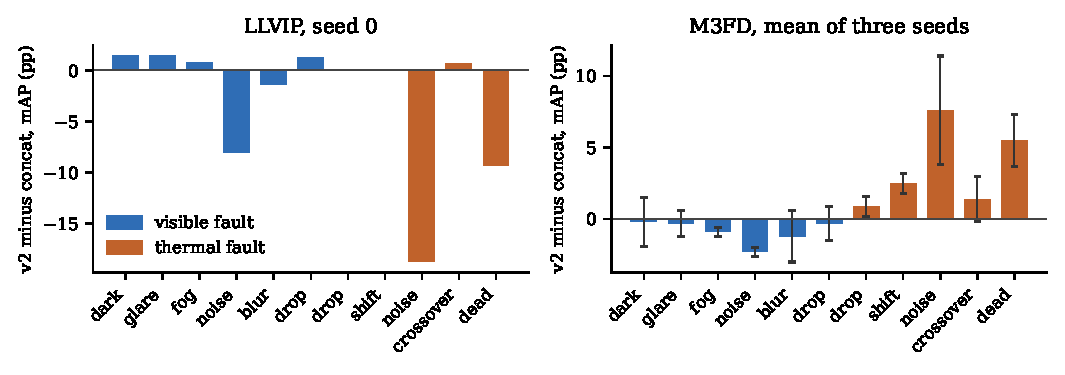
\includegraphics[width=0.85\textwidth]{figures/fig_fault_margin.pdf}
\caption{Margin of CFFM-Net v2 over the concat baseline for each fault at severity three, in mAP points, from Table~\ref{tab:fault}. Positive means v2 is ahead. LLVIP is one seed; M3FD shows the mean over three seeds with the sample standard deviation as an error bar.}
\label{fig:faultmargin}
\end{figure*}

\subsection{Ablations and the negative result}
\label{sec:ablation}
Supplementary Tables~S5 and~S6 list every variant and the margin over the control in each round. Three findings stand out.

First, round one was negative. CFFM-Net v1 had a margin of \marLlvipVoneVsConcatPlainSeedZeroMap{}\,pp on LLVIP and \marMfdVoneVsConcatPlainSeedZeroMap{}\,pp on M3FD against the concat baseline. Part of the gap came from the stride-4 level: adding that head lowers the concat baseline itself from \resLlvipConcatPlainSeedZeroMap{} to \resLlvipConcatPtwoSeedZeroMap{} on LLVIP, and against the concat baseline with the same head, the margin of v1 is \marLlvipVoneVsConcatPtwoSeedZeroMap{}\,pp. We dropped the stride-4 level in v2 on that basis, a decision made on LLVIP at seed zero, since the P2 ablations were not run on M3FD. Removing the gate costs v1 \marLlvipVoneVsVoneNogateSeedZeroMap{}\,pp and replacing the scan by a gated convolution of matched cost \marLlvipVoneVsVoneGconvSeedZeroMap{}\,pp, both within the noise of one seed. We therefore do not claim that the scan or the gate, on their own, explain the v2 gain; the v2 comparison is between complete systems.

Second, v2 recovered the deficit. With three levels and modality dropout, shared by the baseline, v2 is level on LLVIP and ahead on M3FD.

Third, v3 failed in a preliminary, single-seed result. Adding fault training and the reliability loss gives \resLlvipCffmVthreeSeedZeroMap{} mAP on LLVIP and \resMfdCffmVthreeSeedZeroMap{} on M3FD, below v2 on both (\marLlvipVthreeVsVtwoSeedZeroMap{} and \marMfdVthreeVsVtwoSeedZeroMap{}\,pp) and below the fault-trained concat baseline (\marLlvipVthreeVsConcatFtSeedZeroMap{} and \marMfdVthreeVsConcatFtSeedZeroMap{}\,pp). The informative control is v3 without the reliability branch, which keeps the fault training and removes the loss. It reaches \resLlvipCffmVthreeNorelSeedZeroMap{} on LLVIP and \resMfdCffmVthreeNorelSeedZeroMap{} on M3FD and so v3 minus this control is \marLlvipVthreeVsVthreeNorelSeedZeroMap{} and \marMfdVthreeVsVthreeNorelSeedZeroMap{}\,pp: the branch costs accuracy. We therefore report the reliability loss as a negative ablation and do not include it in the recommended recipe. These are single-seed runs, so the size of the effect is uncertain, but the sign agrees on both datasets. A plausible cause is that the loss pushes the mean reliability toward a target that the detection loss does not need, and the two objectives compete. We did not test that explanation.

\subsection{Cost}
\label{sec:cost}
Table~\ref{tab:latency} gives the cost of the evaluated models on a \latLocalDevice{}, in half precision at batch one, timed on an otherwise idle GPU. CFFM-Net v2 has \latLocalVtwoParamsM{}\,M parameters and \latLocalVtwoGflops{} GFLOPs, a median latency of \latLocalVtwoMedianMs{}\,ms (about \latLocalVtwoFps{} frames per second) and a 95th percentile of \latLocalVtwoPNinetyFiveMs{}\,ms. Against the concat baseline this is \latLocalRatioParams{} times the parameters, \latLocalRatioGflops{} times the FLOPs, \latLocalRatioMedian{} times the median latency and \latLocalRatioPNinetyFive{} times the 95th-percentile latency, so v2 passes the limit of at most twice the baseline latency that was fixed in advance. Against the thermal-only detector the median latency is \latLocalVtwoOverThmMedian{} times higher. v3 and its no-branch control have the size of v2, and v3 is \latLocalVthreeOverVtwoMedian{} times the median latency of v2 in this run, so the timing differences between these three models are small and partly noise.

\begin{table}[t]
\centering
\caption{Parameters (millions), GFLOPs and latency (ms) on a \latLocalDevice{}, half precision, batch one, \cfgLatW{}$\times$\cfgLatH{} input, median and 95th percentile per image over \cfgLatIters{} timed iterations after \cfgLatWarmup{} warm-up iterations, on an otherwise idle GPU.}
\label{tab:latency}
{\footnotesize\setlength{\tabcolsep}{4pt}
\begin{tabular}{lrrrr}
\toprule
Model & Params & GFLOPs & Median & p95 \\
\midrule
YOLO26-n thermal only & \latLocalYoloThmParamsM & \latLocalYoloThmGflops & \latLocalYoloThmMedianMs & \latLocalYoloThmPNinetyFiveMs \\
Concat, modality dropout & \latLocalConcatMdParamsM & \latLocalConcatMdGflops & \latLocalConcatMdMedianMs & \latLocalConcatMdPNinetyFiveMs \\
Concat, fault training & \latLocalConcatFtParamsM & \latLocalConcatFtGflops & \latLocalConcatFtMedianMs & \latLocalConcatFtPNinetyFiveMs \\
CFFM-Net v2 & \latLocalVtwoParamsM & \latLocalVtwoGflops & \latLocalVtwoMedianMs & \latLocalVtwoPNinetyFiveMs \\
v3, no reliability branch & \latLocalVthreeNorelParamsM & \latLocalVthreeNorelGflops & \latLocalVthreeNorelMedianMs & \latLocalVthreeNorelPNinetyFiveMs \\
CFFM-Net v3 & \latLocalVthreeParamsM & \latLocalVthreeGflops & \latLocalVthreeMedianMs & \latLocalVthreePNinetyFiveMs \\
\midrule
v2 over concat, ratio & \latLocalRatioParams & \latLocalRatioGflops & \latLocalRatioMedian & \latLocalRatioPNinetyFive \\
\bottomrule
\end{tabular}}
\end{table}


\subsection{Context with published detectors}
\label{sec:sota}
The experiments above compare CFFM-Net with a matched baseline and not with published fusion detectors, because published numbers differ in backbone, input size, training schedule, annotations and split. Tables~\ref{tab:sota} and~\ref{tab:sotakaist} nevertheless place our results next to those figures, copied from the cited papers and not re-run, so that a reader can see the distance. Our models are nano scale: CFFM-Net v2 has \latLocalVtwoParamsM{}\,M parameters and \latLocalVtwoGflops{} GFLOPs at $\cfgLatW{}\times\cfgLatH{}$, and runs at a median of \latLocalVtwoMedianMs{}\,ms on a laptop GPU. We make no claim about relative efficiency.

\begin{table*}[t]
\centering
\caption{Published RGB-T detection results for context, in percent. Numbers are copied from the cited papers, not re-run. Input size or split is stated per row because mAP depends on both. Our models are nano scale, trained on one third of the LLVIP training frames (mean of three seeds), so they are not a like-for-like comparison. On M3FD no row shares a split with ours, and no ranking is claimed.}
\label{tab:sota}
{\footnotesize\setlength{\tabcolsep}{4pt}
\begin{tabular}{lllcc}
\toprule
Method & Detector & Input or split & mAP$_{50}$ & mAP \\
\midrule
\multicolumn{5}{l}{\emph{LLVIP, official split (12,025 / 3,463 pairs)}} \\
YOLOv5-l, infrared only~\cite{jia2021llvip} & YOLOv5-l & not stated & 96.5 & 67.0 \\
CFT~\cite{fang2021cft} & YOLOv5 with CFB & 640$\times$640 & 97.5 & 63.6 \\
CSSA~\cite{cao2023csaa} & Faster R-CNN, ResNet-50 & 640$\times$512 & 94.3 & 59.2 \\
MS-DETR~\cite{xing2024msdetr} & Deformable DETR, ResNet-50 & 640$\times$512 & 97.9 & 66.1 \\
Fusion-Mamba~\cite{dong2025fusionmamba} & YOLOv8-l & 640$\times$640 & 97.0 & 64.3 \\
DAMSDet~\cite{guo2024damsdet} & DETR, ResNet-50 & 1024$\times$1024 & 97.9 & 69.6 \\
TFDet~\cite{zhang2024tfdet} & YOLOv5-l & not stated & 97.9 & 71.1 \\
WaveMamba~\cite{zhu2025wavemamba} & YOLOv8 & not stated & 98.3 & 66.0 \\
IRDFusion~\cite{shen2025irdfusion} & Co-DETR & 640$\times$640 & 98.4 & 70.9 \\
CFFM-Net v2 (this work) & YOLO26-n, \latLocalVtwoParamsM{}\,M & \cfgImgsz{}, every third frame & \resLlvipCffmVtwoMeanMapFifty & \resLlvipCffmVtwoMeanMap \\
Concat baseline (this work) & YOLO26-n, \latLocalConcatMdParamsM{}\,M & \cfgImgsz{}, every third frame & \resLlvipConcatMdMeanMapFifty & \resLlvipConcatMdMeanMap \\
\midrule
\multicolumn{5}{l}{\emph{M3FD, splits differ between rows and are not comparable}} \\
TarDAL, fused image~\cite{liu2022tardal} & YOLOv5 & 3,500 train, test not stated & 80.7 & -- \\
DAMSDet~\cite{guo2024damsdet} & DETR, ResNet-50 & 3,368 / 831, by scene & 80.2 & 52.9 \\
TFDet~\cite{zhang2024tfdet} & YOLOv5 & 2,905 / 1,295 & 64.8 & 41.0 \\
E2E-MFD~\cite{zhang2024e2emfd} & Detectron2, end to end & 2,940 / 1,260 & 91.8 & 63.8 \\
Fusion-Mamba~\cite{dong2025fusionmamba} & YOLOv8-l & split of Liang et al. & 88.0 & 61.9 \\
WaveMamba~\cite{zhu2025wavemamba} & YOLOv8 & 3,360 / 840 & 92.1 & 64.4 \\
CFFM-Net v2 (this work) & YOLO26-n, \latLocalVtwoParamsM{}\,M & 3,360 / 840, random & \resMfdCffmVtwoMeanMapFifty & \resMfdCffmVtwoMeanMap \\
Concat baseline (this work) & YOLO26-n, \latLocalConcatMdParamsM{}\,M & 3,360 / 840, random & \resMfdConcatMdMeanMapFifty & \resMfdConcatMdMeanMap \\
\bottomrule
\end{tabular}}
\end{table*}

\begin{table*}[t]
\centering
\caption{KAIST log-average miss rate in percent on the reasonable subset (lower is better). Published rows use the improved test annotations and the standard evaluation code and are copied from the cited papers. Our rows use the original annotations for training and testing, every 20th test frame and our own implementation of the protocol, so they are indicative only.}
\label{tab:sotakaist}
{\footnotesize\setlength{\tabcolsep}{4pt}
\begin{tabular}{lllccc}
\toprule
Method & Detector & Train annotations & All & Day & Night \\
\midrule
AR-CNN~\cite{zhang2019arcnn} & VGG-16 & sanitized & 9.34 & 9.94 & 8.38 \\
MBNet~\cite{zhou2020mbnet} & ResNet-50 & AR-CNN improved & 8.13 & 8.28 & 7.86 \\
GAFF, original training~\cite{zhang2021gaff} & VGG-16 & original & 10.62 & 10.82 & 10.14 \\
GAFF, sanitized training~\cite{zhang2021gaff} & VGG-16 & sanitized & 6.48 & 8.35 & 3.46 \\
ICAFusion~\cite{shen2024icafusion} & YOLOv5, CSPDarknet53 & sanitized & 7.17 & 6.82 & 7.85 \\
MS-DETR~\cite{xing2024msdetr} & ResNet-50 & sanitized & 6.13 & 7.78 & 3.18 \\
TFDet~\cite{zhang2024tfdet} & VGG-16 & sanitized & 4.47 & 5.22 & 3.36 \\
\midrule
Concat baseline (this work) & YOLO26-n & original & \kstConcatAllMr & \kstConcatDayMr & \kstConcatNightMr \\
CFFM-Net v2 (this work) & YOLO26-n & original & \kstCffmAllMr & \kstCffmDayMr & \kstCffmNightMr \\
\bottomrule
\end{tabular}}
\end{table*}


On LLVIP, with the official split, v2 reaches \resLlvipCffmVtwoMeanMapFifty{}\,\% mAP$_{50}$ and \resLlvipCffmVtwoMeanMap{}\,\% mAP, in the range of published fusion results (mAP from \sotaLlvipFusionMapMin{} to \sotaLlvipFusionMapMax{}) and below the best of them. This is with training on one third of the training frames and without a large backbone. The comparison is weaker than it looks. The LLVIP infrared-only baseline with a large YOLOv5 already reaches \sotaLlvipIrOnlyMap{} mAP in the dataset paper~\cite{jia2021llvip}, so thermal imagery alone nearly saturates the benchmark, and a gap of a few points of mAP between two fusion detectors at different input sizes (one row trains at a much larger input than the others) says little about the fuser. On M3FD no row shares our split. Published values of mAP$_{50}$ run from \sotaMfdMapFiftyMin{} to \sotaMfdMapFiftyMax{} across splits of the same dataset, and the same method (CFT) is reported \sotaMfdSplitSwing{} points of mAP$_{50}$ apart in two cited papers that use different splits, so we draw no ranking from the M3FD rows.

On KAIST our miss rates are far above the published ones (Table~\ref{tab:sotakaist}): \kstConcatAllMr{}\,\% for the concat baseline and \kstCffmAllMr{}\,\% for CFFM-Net v2 against \sotaKaistMrMin{} to \sotaKaistMrMax{} for the published detectors, which use ResNet or VGG backbones, sanitised training annotations and the standard evaluation code. We attribute part of the gap to the protocol differences in Section~\ref{sec:kaistprotocol} and part to scale and a short schedule, but we did not run the experiments that would apportion it, and the table should be read as showing that our KAIST detectors are not competitive with the published state of the art. The KAIST experiments serve the video questions of Section~\ref{sec:video} and not a leaderboard claim.

\subsection{What the gate learns}
\label{sec:gate}
Figure~\ref{fig:trust} plots, for LLVIP and M3FD test images, the share of fusion weight given to the thermal camera against the mean brightness of the visible image, for a round-one model. The share moves in the expected direction. In the darkest LLVIP scenes it leans toward thermal and in the brightest M3FD scenes toward visible. The swing is small, and the share stays close to one half everywhere. The gate at round one is therefore a mild prior and not a switch, which fits the modest gains above. Figure~\ref{fig:hero} shows the trust map on one night scene.

\begin{figure*}[t]
\centering
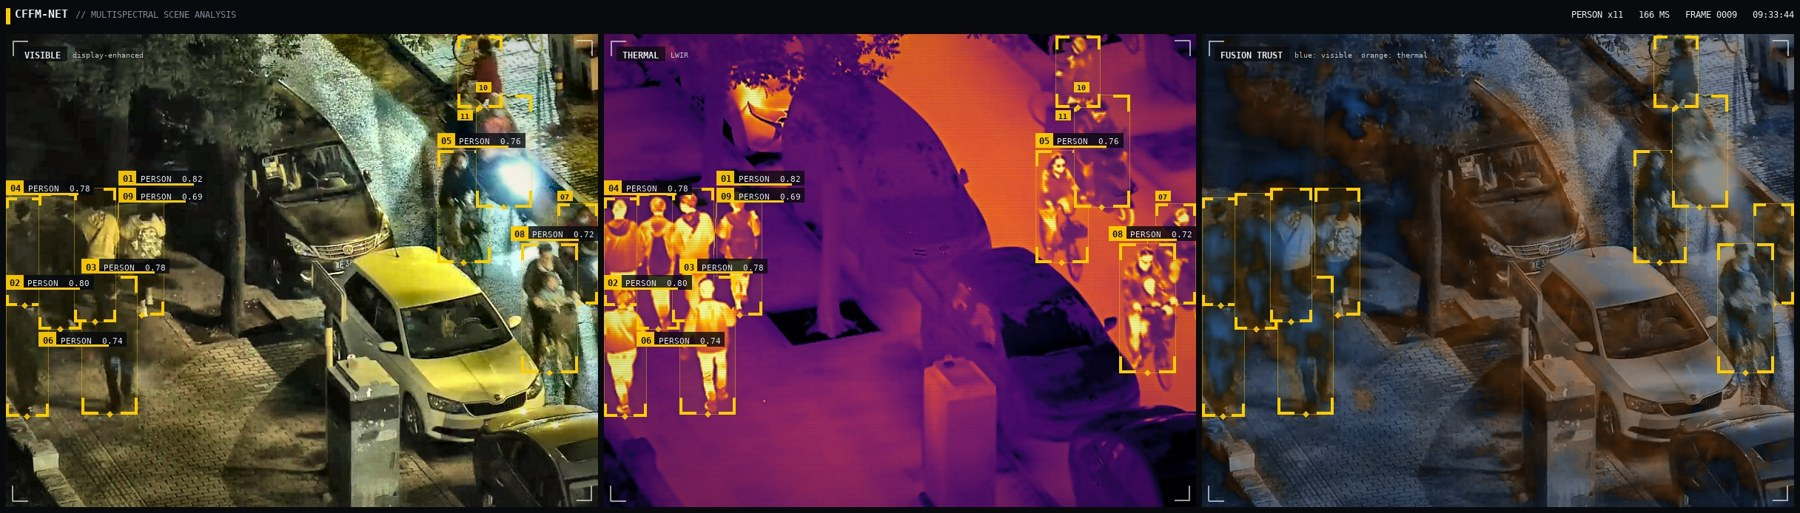
\includegraphics[width=0.9\textwidth]{figures/hero_llvip.jpg}
\caption{A LLVIP test pair as the round-one CFFM-Net sees it: visible with detections, thermal, and the fusion trust map in which blue marks visible and orange marks thermal weight.}
\label{fig:hero}
\end{figure*}

\begin{figure}[t]
\centering
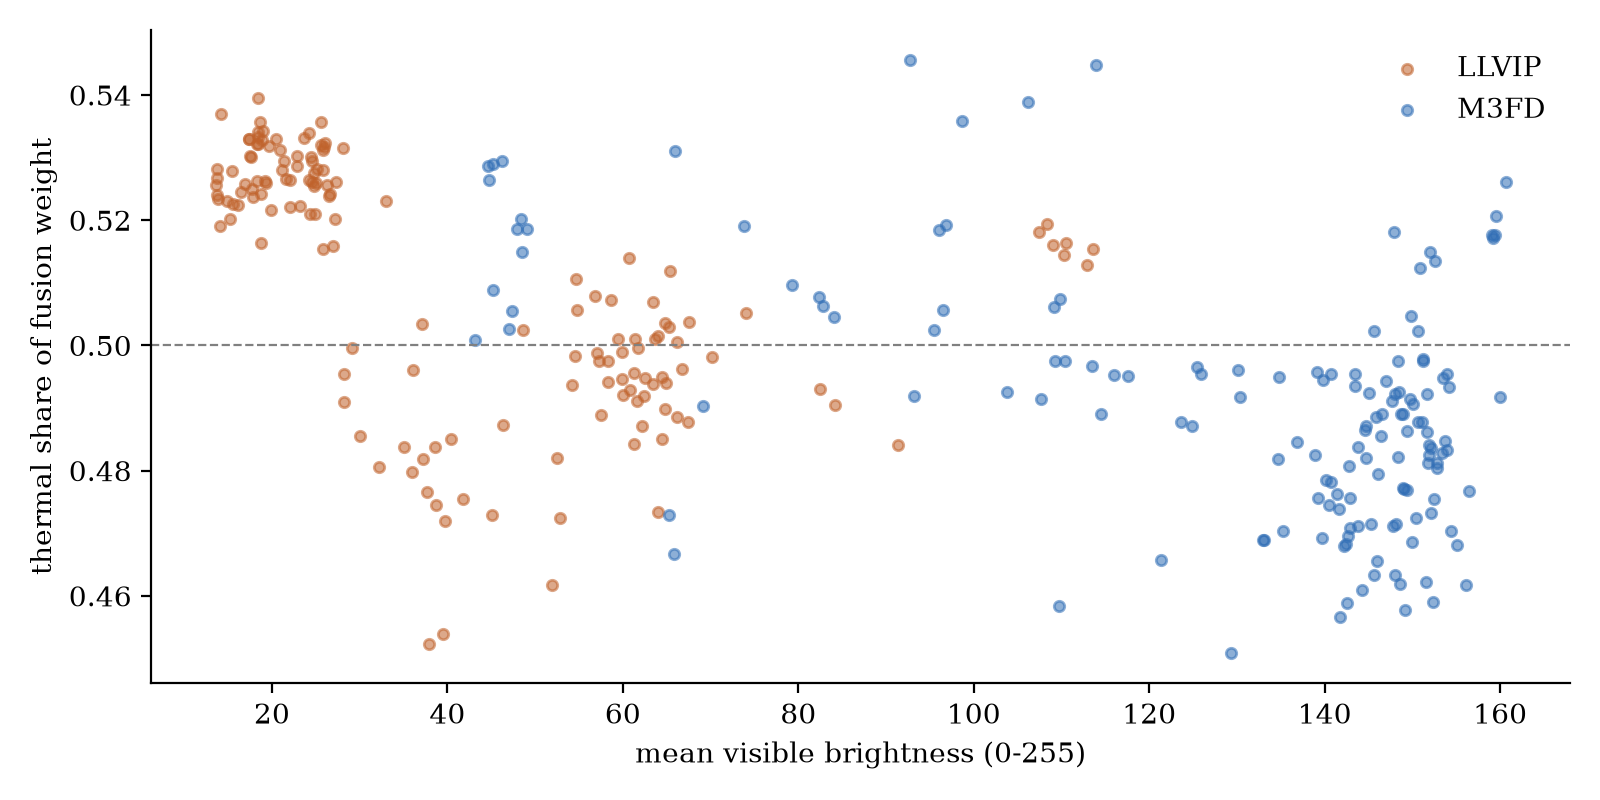
\includegraphics[width=\columnwidth]{figures/trust_vs_brightness.png}
\caption{Thermal share of the fusion weight against mean visible brightness for LLVIP and M3FD test images, with a round-one CFFM-Net. The dashed line marks an equal share.}
\label{fig:trust}
\end{figure}
